\frame{
    \frametitle{Track Quality Values}

    Track quality values appear to have no effect on performance at all

    \begin{columns}[T]
        \begin{column}{0.33\textwidth}
            \begin{figure}
                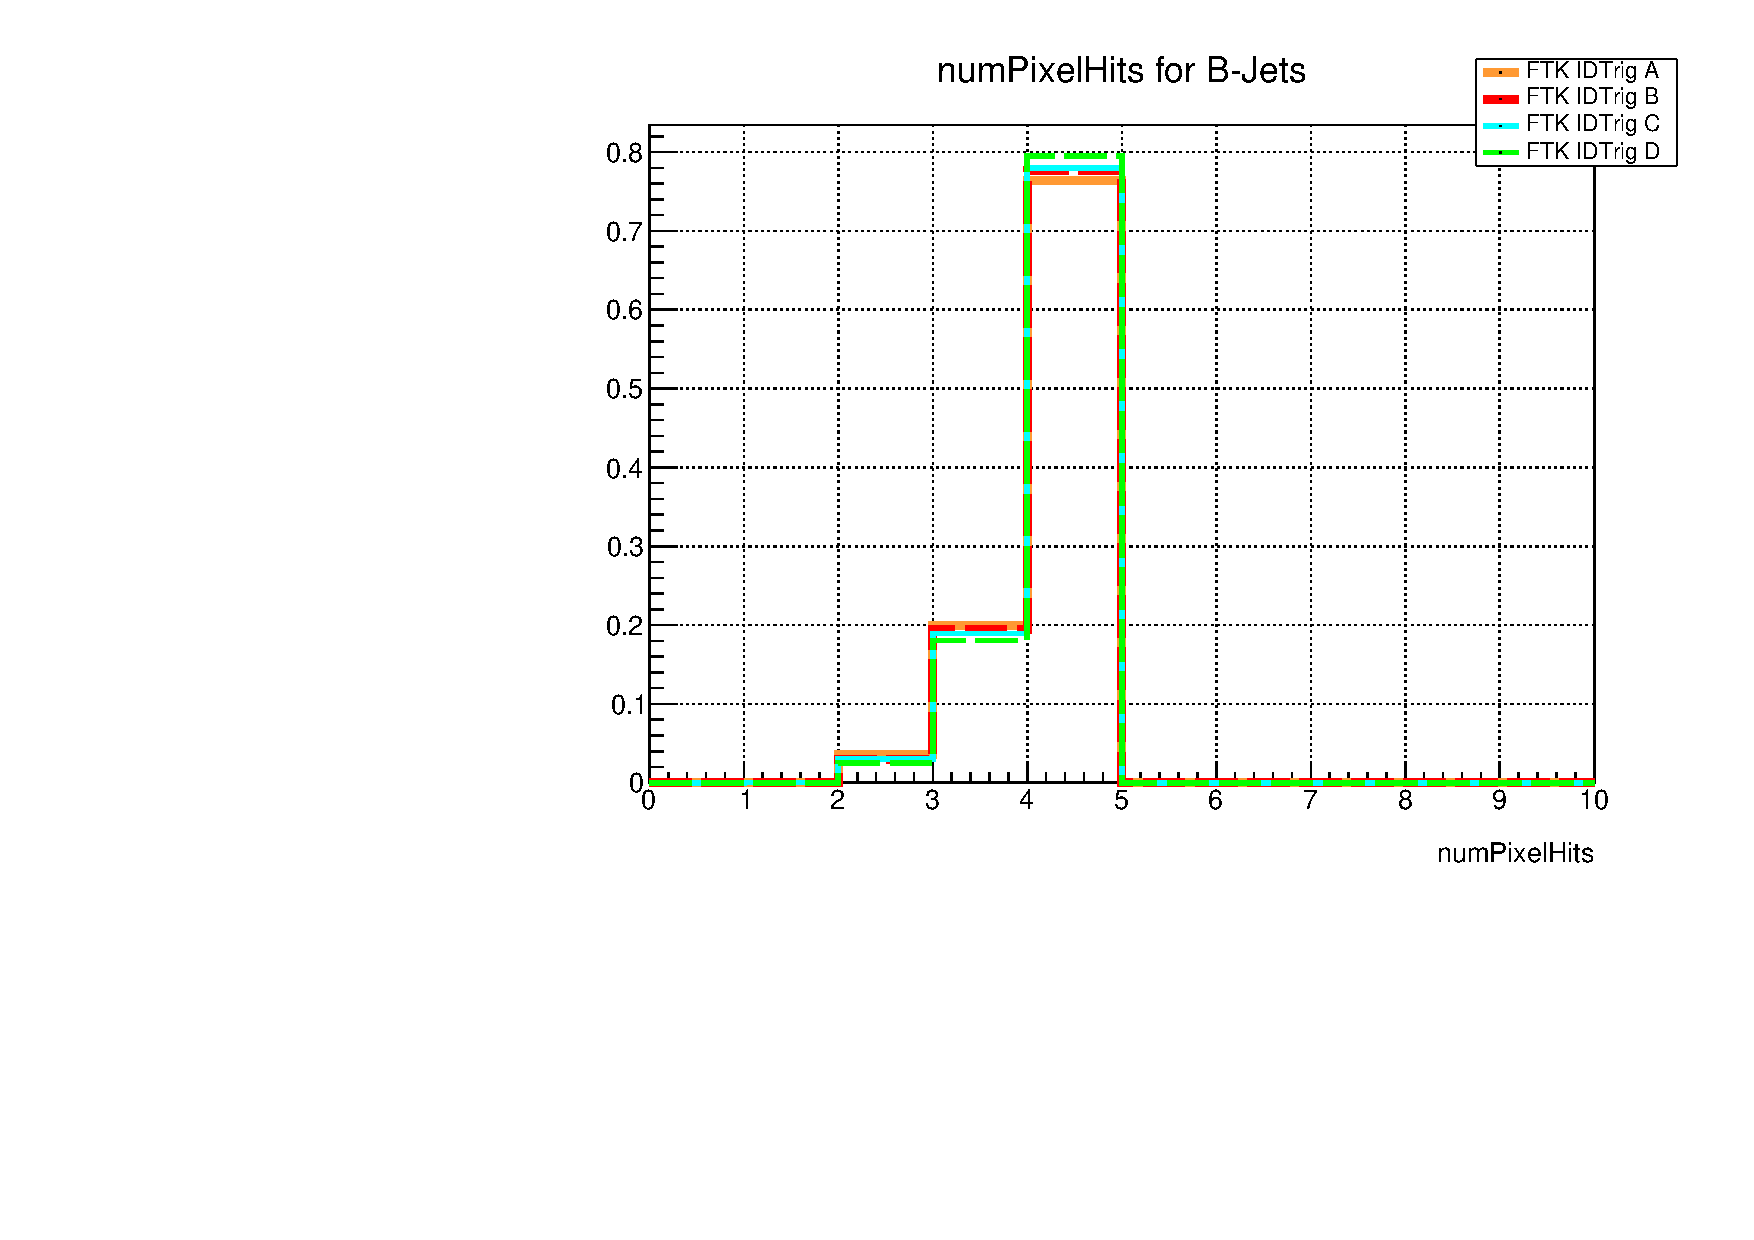
\includegraphics
                [width=\linewidth,height=\textheight,keepaspectratio]
                {correlation_numPixelHits_0}
            \end{figure}
            \begin{figure}
                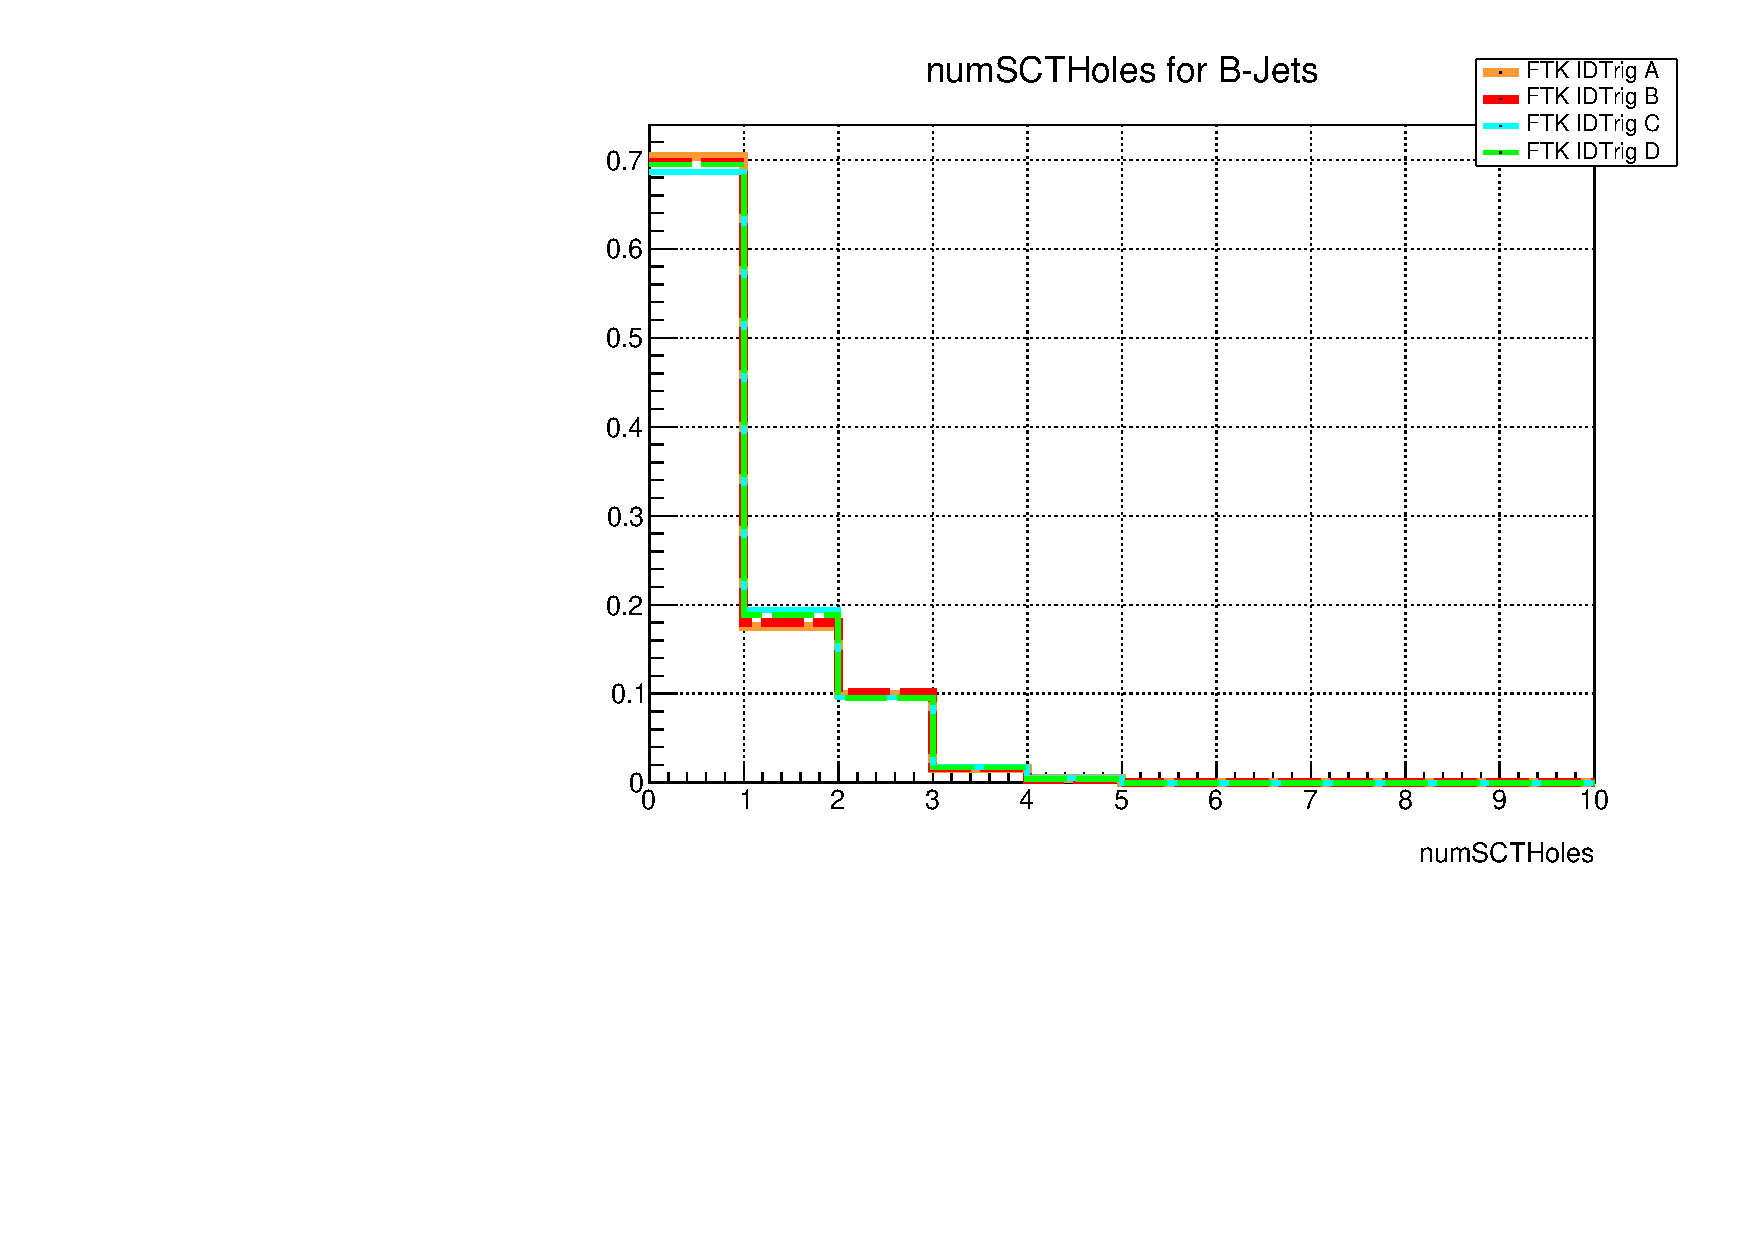
\includegraphics
                [width=\linewidth,height=\textheight,keepaspectratio]
                {correlation_numSCTHoles_0}
            \end{figure}
        \end{column}
        \begin{column}{0.33\textwidth}
            \begin{figure}
                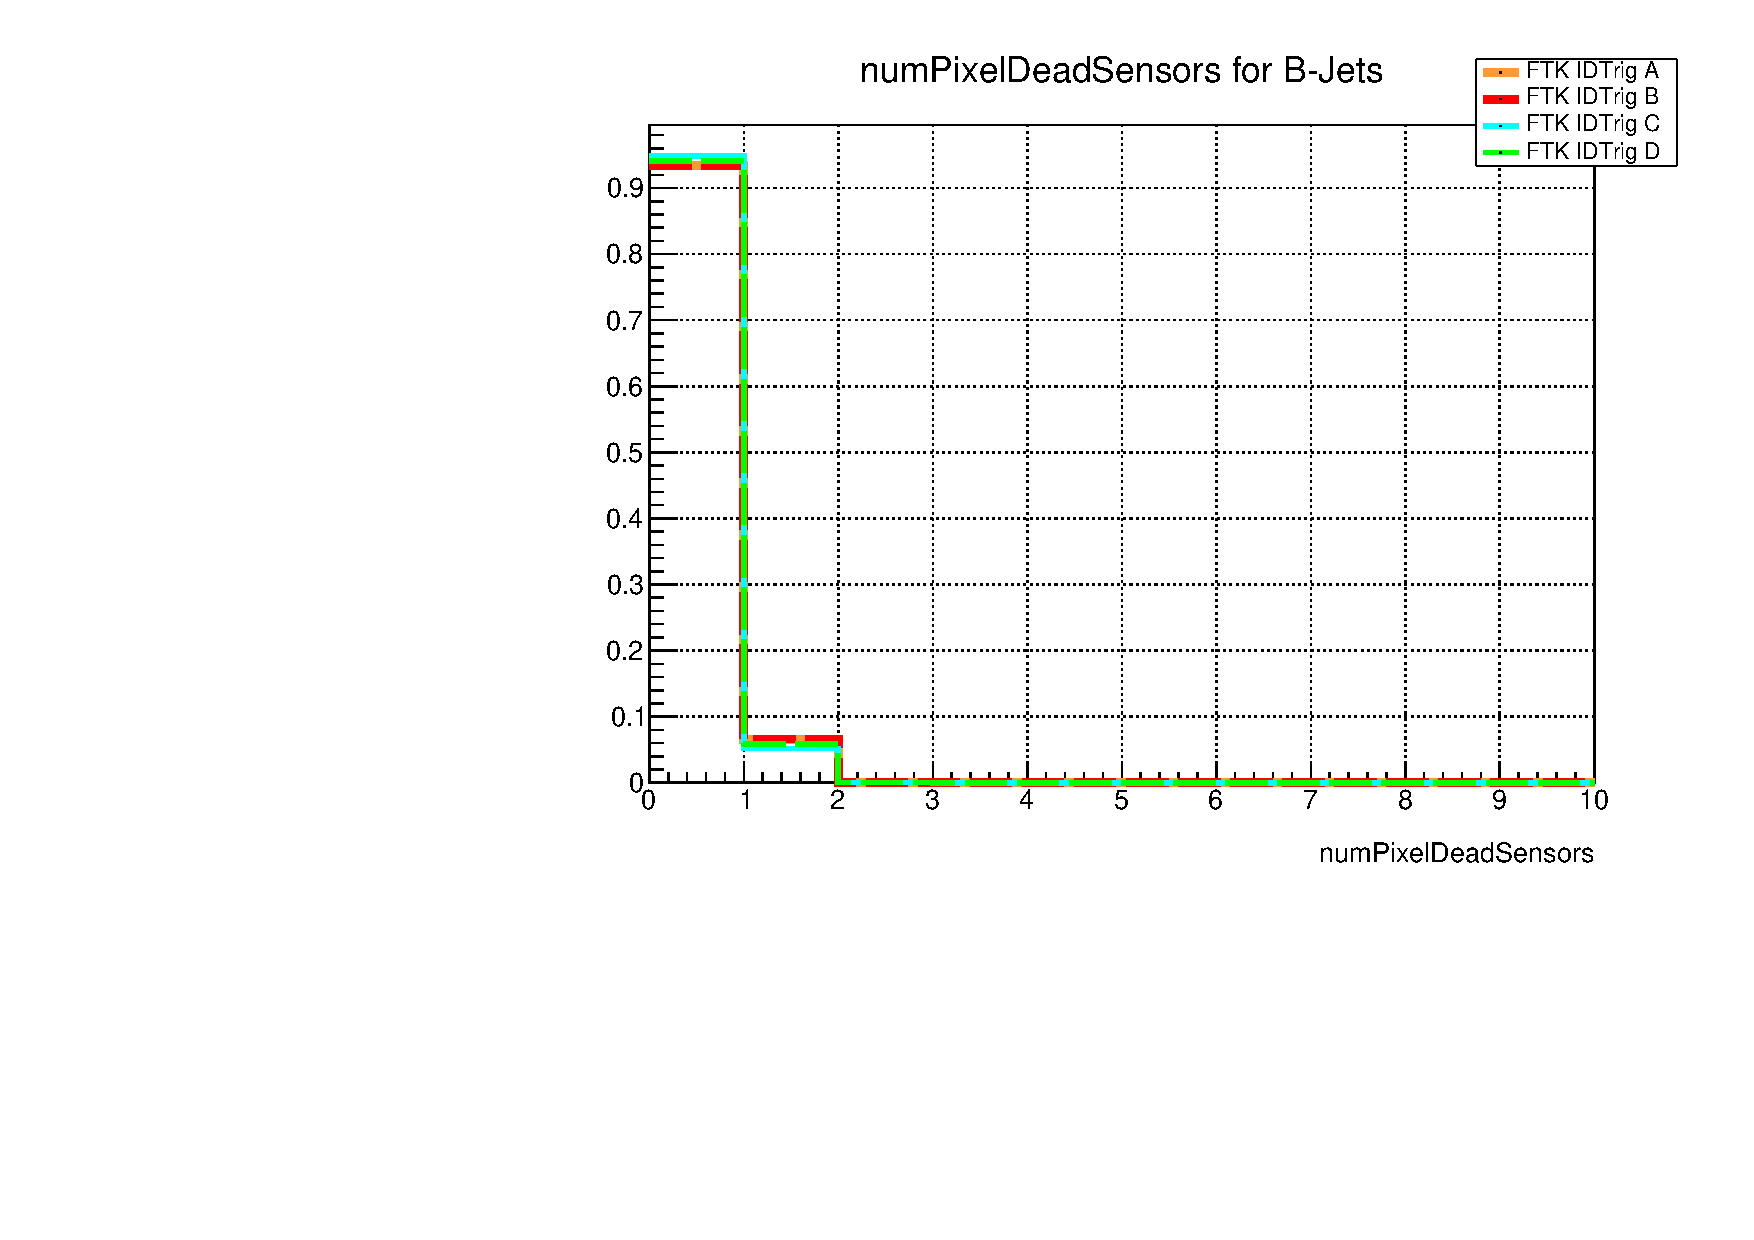
\includegraphics
                [width=\linewidth,height=\textheight,keepaspectratio]
                {correlation_numPixelDeadSensors_0}
            \end{figure}
            \begin{figure}
                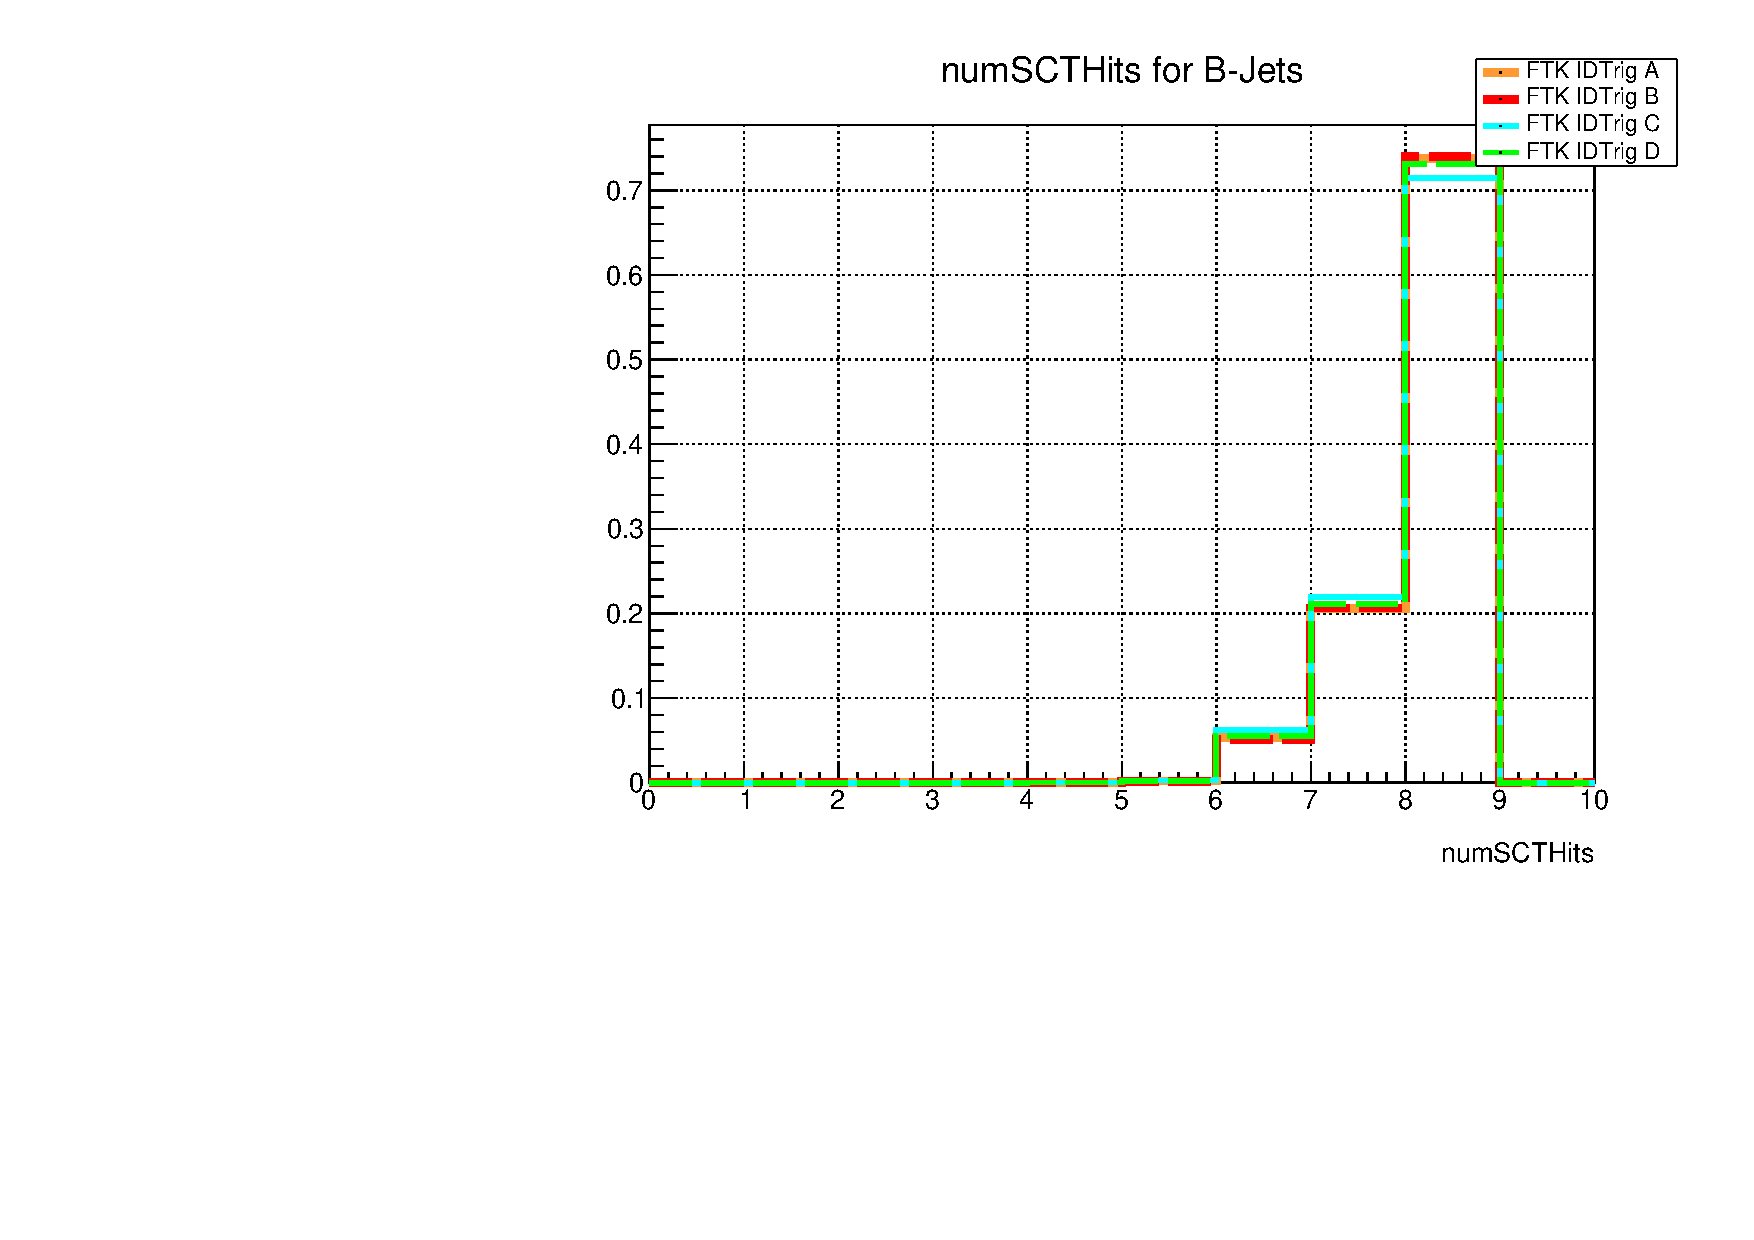
\includegraphics
                [width=\linewidth,height=\textheight,keepaspectratio]
                {correlation_numSCTHits_0}
            \end{figure}
        \end{column}
        \begin{column}{0.33\textwidth}
            \begin{figure}
                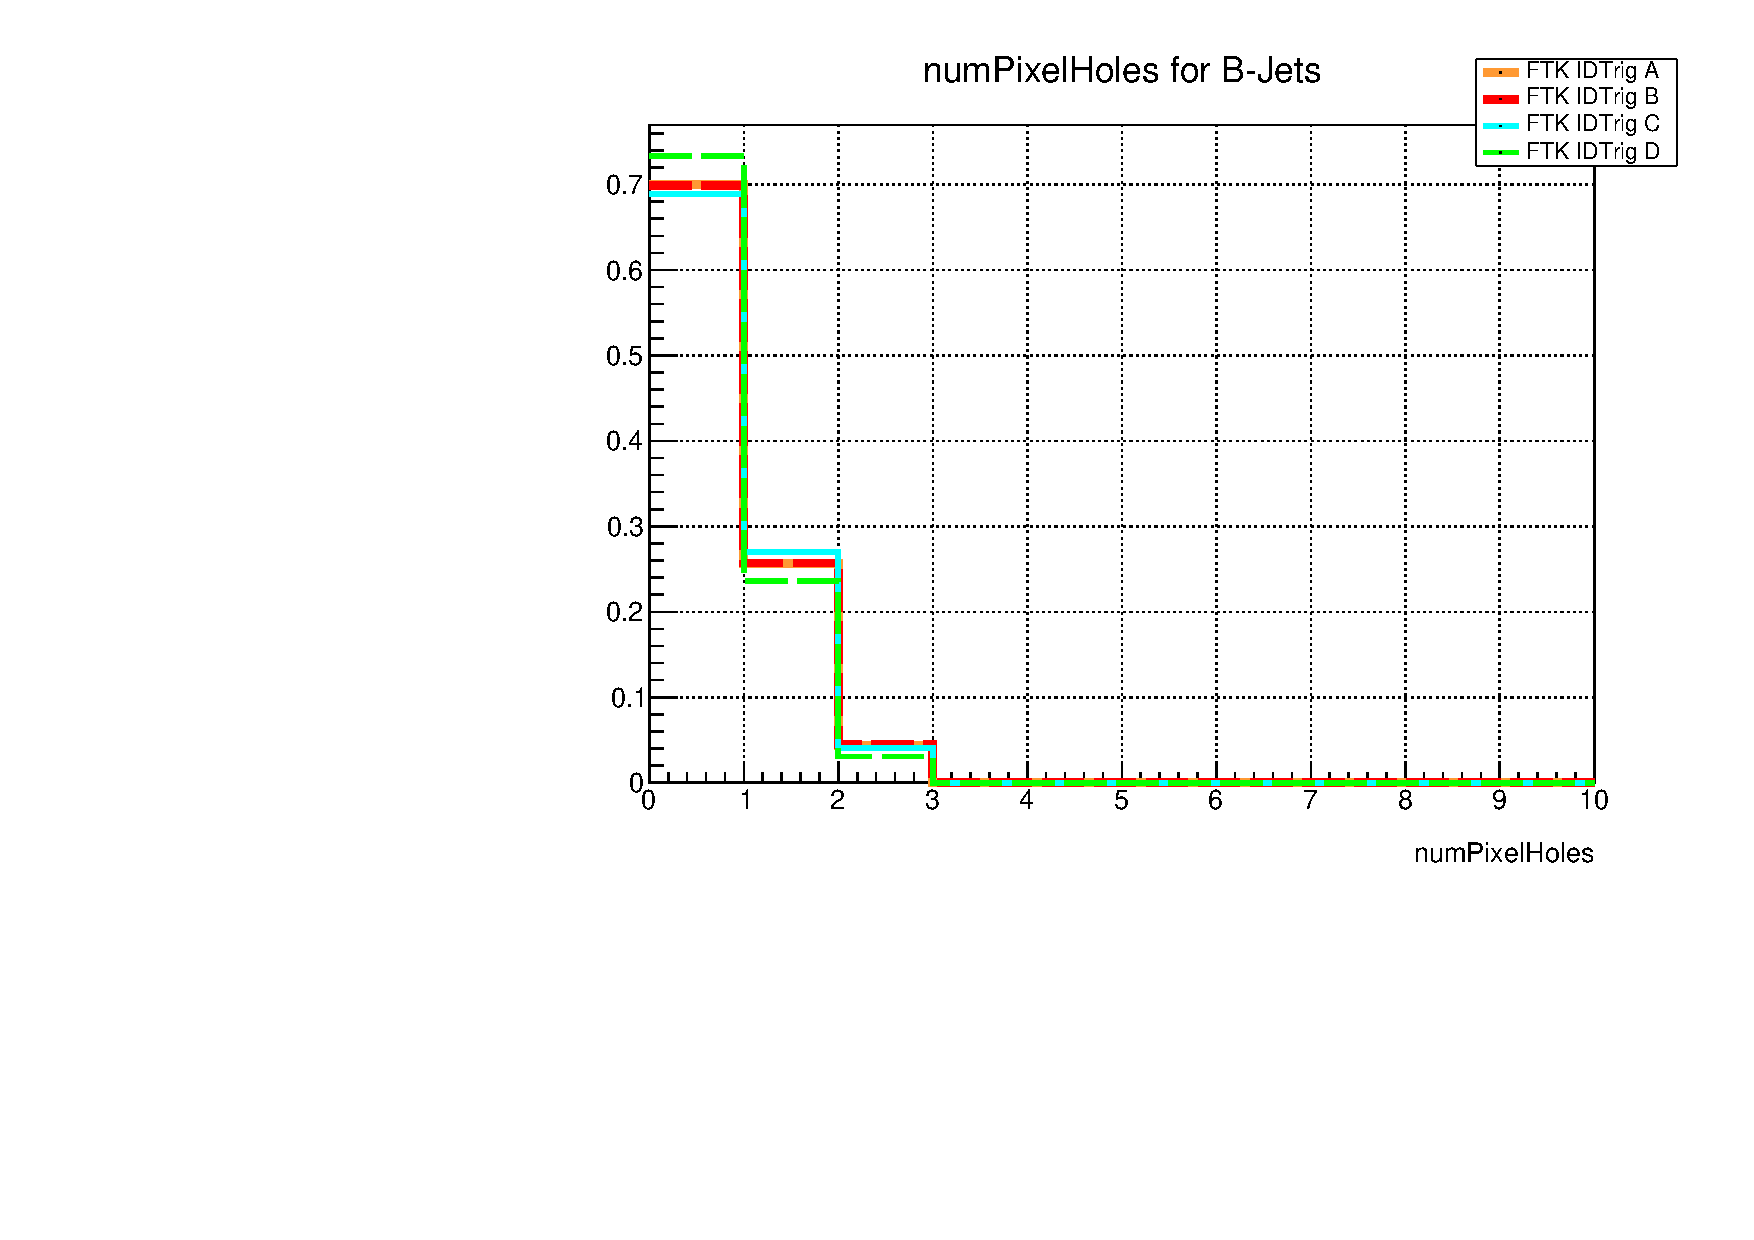
\includegraphics
                [width=\linewidth,height=\textheight,keepaspectratio]
                {correlation_numPixelHoles_0}
            \end{figure}
            \begin{figure}
                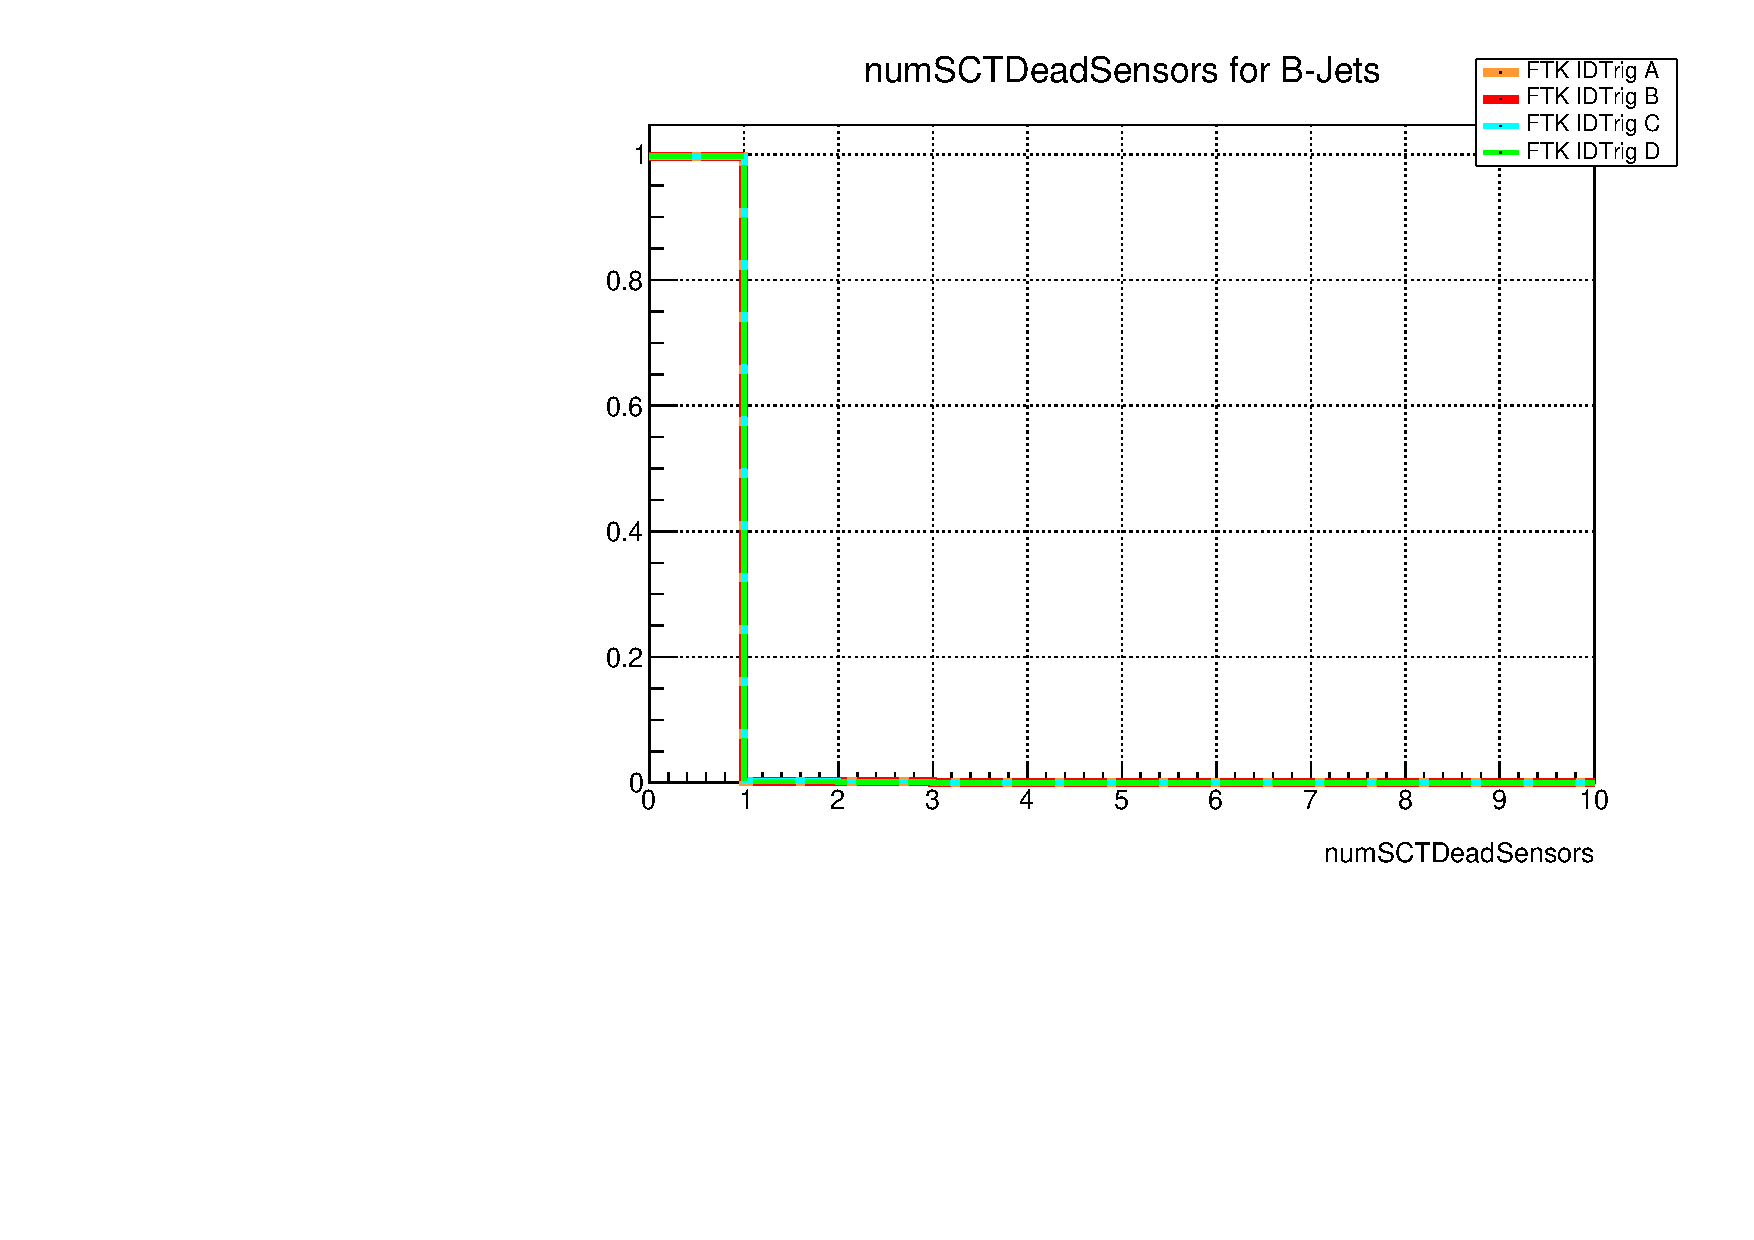
\includegraphics
                [width=\linewidth,height=\textheight,keepaspectratio]
                {correlation_numSCTDeadSensors_0}
            \end{figure}
        \end{column}
    \end{columns}
}

\displaythree{ Track $\theta$ Jet by Jet Performance, FTK Distribution }
    {\small \vspace{30pt} Uniquely, the FTK appears to have improved performance over the HLT
        in low $\theta$ tracks}
    {track_study/plot_ftk_correlation_theta_0}
    {track_study/plot_ftk_correlation_theta_err_0}
    {track_study/plot_ftk_correlation_theta_sig_0}
